
\begin{dialog}{三部创意曲}

\begin{quote}
阿基里斯\lnote{(希腊的一位勇士,长着一双飞毛腿,是跑得最快的人)}和一只乌龟这时一同站在骄阳下满是尘土的跑道上。跑道的另一头有一根高高的旗杆,上面挂着一面长方形的大旗,整个旗子都是红色的,只是上面开有一个环状的狭缝,透过它可以看见天空。
\end{quote}

\begin{dialogue}

\item[阿基里斯]跑道那头儿是面什么旗子啊?这叫我想起我最喜欢的艺术家艾舍尔画的一幅版画。

\item[乌龟]那是芝诺的旗子。

\item[阿基里斯]这面旗子上的那个孔和艾舍尔画的莫比乌斯带上的孔差不多吧?我看得出,那旗子有点毛病。

\begin{figure}[!htb]
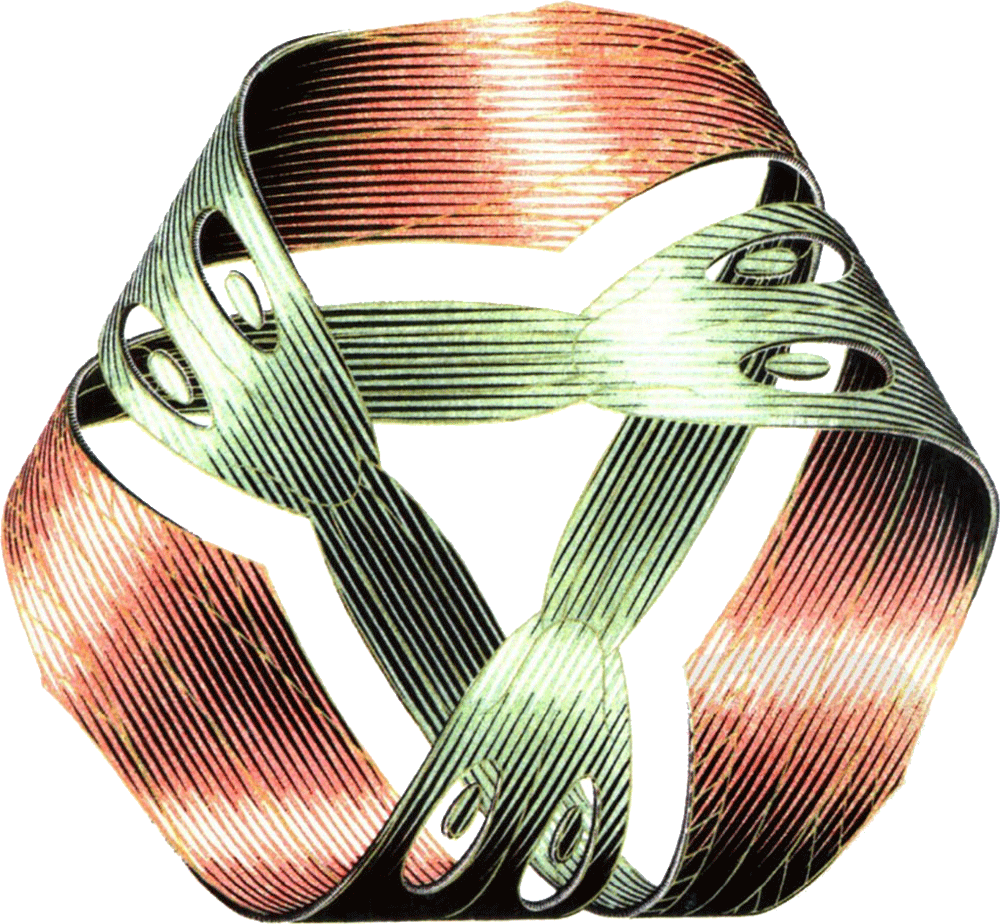
\includegraphics{img_010.png}
\caption[莫比乌斯带I,艾舍尔作。]
  {莫比乌斯带I,艾舍尔作(四版套印木刻,1961)。}
\end{figure}

\item[乌龟]从旗子上切下的环呈阿拉伯数字“零”的形状,芝诺最喜欢这个数字。

\item[阿基里斯]可是“零”现在还没发明出来呢!这得在大约一千年以后,由印度的一位数学家把它发明出来。因此,龟兄,我的论据证明这面旗子是不可能的。

\item[乌龟]你这论据很有说服力,阿基,我不得不同意,这样的旗子确实是不可能的。可是不管怎么说,它很漂亮,不是吗?

\item[阿基里斯]哦,是啊,它很美,这是毫无疑问的。

\item[乌龟]我疑心它的美是否跟它的不可能性有关,这问题我说不好。我从来没有分析过美。什么是美是个很重大的问题,而我似乎从来没有考虑过这种重大的问题。

\item[阿基里斯]说到重大的问题,龟兄,你思考过生活的目的没有?

\item[乌龟]噢,天哪,没有。

\item[阿基里斯]你是否想过我们为什么在此存在,或者说,是谁创造了我们?

\item[乌龟]哦,这完全是另一回事。我们俩都是芝诺创造的(这一点不久你就会明白);我们俩之所以呆在这儿是因为要进行一次赛跑。

\item[阿基里斯]赛跑?多荒唐啊!我这个长着一双飞毛腿的世界上跑得最快的人和你这个爬得不能再慢的家伙赛跑?这种比赛毫无意义!

\item[乌龟]你可以让我先跑一段嘛。

\item[阿基里斯]那得是很长的一段。

\item[乌龟]我不反对。

\item[阿基里斯]不过迟早我会追上你的。很可能不会太迟。

\item[乌龟]要是事情按芝诺的悖论发展,你就追不上。你知道,芝诺想用你我的赛跑来表明运动是不可能的。照芝诺的说法,只是在人们的头脑中,运动才显得可能,而实际上,运动从本质上说是不可能的。他的证明很漂亮。

\item[阿基里斯]哦,对了,现在我想起来了:那个著名的关于禅师芝诺的禅宗公案,正像你所说的,确实很简单。

\item[乌龟]禅宗公案?禅师?你想说什么?

\item[阿基里斯]是这样:两个和尚围绕着一面旗幡的问题争论起来,一个说“幡动”,另一个说“风动”。六祖芝诺正巧从这里走过,告诉他们:“风幡非动,心自动耳。”

\item[乌龟]恐怕你弄错了,阿基。芝诺不是什么禅师,根本不是,他其实是个来自爱利亚城(位于$A$点与$B$点中间的地方)的希腊哲学家。几个世纪之后,他将以他的运动悖论闻名于世,你我进行的这场赛跑将在他的一个悖论里扮演重要角色。

\item[阿基里斯]哦,是我弄混了?让我想想那到底是谁的运动悖论:芝诺的?智能的?慧能的?嗨,我脑子里悖论太多,搞不清谁对谁了。\dlnote{(忽然刮过一阵微风。)}——噢,瞧啊,龟兄,那旗子动了!我真喜欢看那柔软的布料上闪烁的波纹!上面挖去的那个环形也在动呢!

\item[乌龟]别犯傻了。旗子本身就是不可能的,更别说它在飘动了,是风在动。

\dnote{(这时正巧芝诺从一旁走过。)}

\item[芝诺]好啊,好啊!怎么回事?怎么啦?

\item[阿基里斯]幡在动。

\item[乌龟]风在动。

\item[芝诺]哦,朋友们!停止你们的争论,抛却你们的讥讽,放弃你们的不和吧!我将帮你们解决这个问题。嘿!在这样一个好天里!

\item[阿基里斯]这家伙一定是蠢货。

\item[乌龟]不,阿基,等等,咱们先听听他想说什么。喂,不知名的先生,恳请您就此发表意见。

\item[芝诺]愿意效劳。既非风动亦非幡动——谁都没动,根本没有什么东西在动。这是因为我发现了一个伟大的定理,这个定理说:“运动从本质上说是不可能的”。从这个定理可以推导出一个更伟大的定理——芝诺定理:“运动无有”。

\item[阿基里斯]“芝诺定理”?先生,您难道就是爰利亚的哲学家芝诺?

\item[芝诺]正是敝人,阿基里斯。

\item[阿基里斯]\dlnote{(疑惑地搔着头)}他怎么知道我的名字?

\item[芝诺]我是否可以请二位听我讲讲事情的经过?我今天下午之所以从$A$点到爱利亚,就是为了找个人,这个人要对我这个经过周密推敲的论证感兴趣。但是人们全都忙忙碌碌的,谁也没有时间。你们不知道一再被人拒绝是件多么令人沮丧的事。哦,很抱歉用这些烦事来打扰你们。我现在只想麻烦二位一件事:二位能让我这个又老又迂的哲学家满足一会儿——只用一小会儿,我担保——让我讲讲我那奇怪的理论?

\item[阿基里斯]哦,完全可以!请给我们讲讲吧!我想我说出了我们俩人的共同愿望,因为我的伙伴乌龟先生刚刚还以非常尊敬的口吻说到您,他特别提到了您的悖论。

\item[芝诺]谢谢。你们知道,我的师傅五祖诲谕我说,真如即一,具有不变异性,森罗万象及动迁变化皆是感官的幻觉。一些人嘲笑他的观点,可我要证明他们的嘲笑是荒唐的。我的论证很简单。我想利用我创造的两个形象来解释它的意义:这就是阿基里斯和一只乌龟。在我的故事里,他们被一个过路人说服去进行一场赛跑,比赛的终点是跑道那头儿的一面在微风中飘动的旗子。因为乌龟跑起来极慢,所以我们假定让它先跑出一段距离,比如说,十丈吧。现在比赛开始了。仅仅几步,阿基里斯就跑到了乌龟出发的地点。

\item[阿基里斯]哈!

\item[芝诺]现在乌龟只在阿基里斯前面两尺的地方。不一会儿,阿基里也到达了这一点。

\item[阿基里斯]嚯!嚯!

\item[芝诺]可是就在那一会儿的功夫里,乌龟又往前跑了一点点。阿基里斯很快也追到了那一点。

\item[阿基里斯]嘿!嘿!嘿!

\item[芝诺]然而就在那一瞬间,乌龟又往前蹭出了一点儿,阿基里斯这时还是在它后面。现在你们看,阿基里斯要想追上乌龟,这种“试试追上我”的游戏就得做无穷次,因此,阿基里斯永远追不上乌龟!

\item[乌龟]嗨!嗨!嗨!嗨!

\item[阿基里斯]嗬……嗬……嗬……嗬……嗬……这个论证我听着像是错了,可又说不出究竟错在哪儿。

\item[芝诺]是个难题吧?这就是我最喜欢的那个悖论。

\item[乌龟]芝诺,请原谅,我认为您这个故事解释的不是这个原理,对吗?您刚刚告诉我们将以(嘿嘿)阿基里斯永远追不上乌龟这个芝诺的“阿基里斯悖论”闻名于几个世纪以后的是什么,但是“运动从本质上讲是不可能的”(以及进而得到的“运动无有”)这一命题是由您的那个“二分悖论”证明的,是吗?

\item[芝诺]噢,惭愧。当然,你是对的。那个悖论讲如果想从$A$点到$B$点,须得先走完$A$到$B$的一半,要走完这一半,又得先走完这一半的一半,以此类推。但是你们看,这两个悖论其实有着共同的味道,坦率地说,我只有这么一个了不起的思想,只是用了不同的表达方法。

\item[阿基里斯]我敢发誓,这些论证有错误,我看不大出错在哪儿,但是它们不可能是正确的。

\item[芝诺]你怀疑我的悖论的正确性?为什么不真的试试?你看见跑道那头儿那面红色的旗子了吗?

\item[阿基里斯]是仿照艾舍尔作品的那面不可能的旗子吗?

\item[芝诺]正是。您和乌龟先生现在就来赛一赛,跑到那儿,怎么样?让乌龟先生先跑……嗯,我不知道——

\item[乌龟]让我十丈怎么样?

\item[芝诺]好,就十丈。

\item[阿基里斯]我无所谓。

\item[芝诺]太好了!太令人兴奋了!这是一次好机会,可以检验检验我那经过严格证明的定理。乌龟先生,请您先到十丈前您的位置上,好吗?

\dnote{(乌龟朝着旗子的方向爬了十丈。)}

都准备好了吗?

\item[乌龟和阿基里斯]准备好了!

\item[芝诺]各就各位!预备!跑!

\end{dialogue}

\end{dialog}
